
\chapter{Implementation}


\section{\ignorespacesSource Code & Screen Shots}

\subsection{Splash Screen}

\begin{wrapfigure}{r}{0.3845\linewidth}
\centering
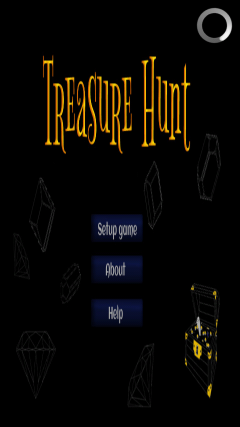
\includegraphics[scale=0.7]{snaps/splash}
\caption{Application Loading}
\label{fig:myfig}
\end{wrapfigure}
\textnormal{Splash Screen is a view that appears for sometimes (3 or 4 seconds).After dislaying splash screen that never comes second time in application until we restart Application.The purpose of a splash screen is to give the user an indication that your app is loading–not to create an extra delay before the user can load your app. People don’t like waiting, especially in a mobile environment.Using Thread,AsyncTask,Handler you can wait sometimes to load your app.The most desirable way to display splash screen is handler.you can do it easily.no need to create thread or async task in your activity.The handler have post Delayed (Runnable,long)  method.using this method you can wait some times to load app.Handler instance is associated with a single thread and that thread's message queue. When you create a new Handler, it is bound to the thread / message queue of the thread that is creating it -- from that point on, it will deliver messages and runnables to that message queue and execute them as they come out of the message queue.

}





%\lstinputlisting{java/splash.java}


\subsection{Location Marker}

\begin{wrapfigure}{r}{0.39\linewidth}
\centering
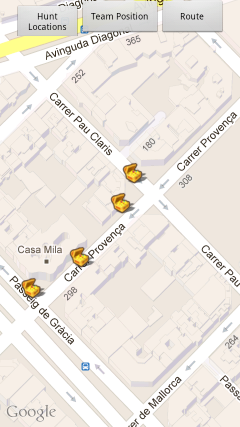
\includegraphics[scale=0.6]{snaps/location}
%\rule{0.9\linewidth}{0.75\linewidth}
\caption{Location Marker Activity}
\label{fig:myfig}
\end{wrapfigure}
\textnormal{
Location Marker is responsible  for plotting the real time location of all the user participating in the game. The functionality is when the player starts the application and registers it,the device starts sending the user co-ordinates to our webserver which is send back to other user using the JSON type in callback which uses the overlays on Android Maps to plot it.

In order to use the Android Maps you need to have maps and its API keys . The Treasure Hunt Icons are saved in the assets folder and the images are scaled for the device screen size and are in the PNG format.Using this Location Marker the user is not only able to see his locations but other locations where the other team are heading .

}

%\lstinputlisting{java/LocationMarker.java}

\subsection{Task List}

Treasure Hunting Game not only remains the concept of hunting treasures with maps but also integrates GPS function. With a designed route for treasure hunting, the students would not miss any places for treasures. During the process of game, students can participate in the activity and observe the environment in person and absorb the knowledge unconsciously. Meanwhile, students can learn how to apply GPS and the skills of reading maps to obtain the knowledge happily.Treasure Hunting Game not only remains the concept of hunting treasures with maps but also integrates GPS function. With a designed route for treasure hunting, the students would not miss any places for treasures. During the process of game, students can participate in the activity and observe the environment in person and absorb the knowledge unconsciously. Meanwhile, students can learn how to apply GPS and the skills of reading maps to obtain the knowledge happily.

\begin{equation*}
  \begin{CD}
    a @>>> b \\
    @VVV @AAA \\
    c @= d
  \end{CD}
  \qquad
  \begin{CD}
    x @>>\alpha> y \\
    @VV\kappa V @A\beta AA \\
    v @<\gamma<< w
  \end{CD}

\end{equation*}

%\lstinputlisting{java/TaskList.java}

\subsection{User Registration}

Treasure Hunting Game can only be played when the user has registered with the server and his device IMSI has been saved on the server,Once the user Installs the Application the user is asked to register the device and select team color , this is achieved using the registration class . A seperate XML layout has been developed for the Registration form . Once the data has been saved the entry is created in Shared Preferences and the application sends the data to webserver , the type of data is UTF-8 and in JSON format

\begin{align*}
\xymatrix@R=10pt{
    cRing \ar[r] & Sch \\
    A \ar@{}[u]|{\rotatebox{90}{$\in$}} \ar@{|->}[r] 
            & Spec(A) \ar@{}[u]|{\rotatebox{90}{$\in$}}
}
\end{align*}



\chapter{Snapshot}

\begin{figure}[h]
\begin{center}$
\begin{array}{cc}
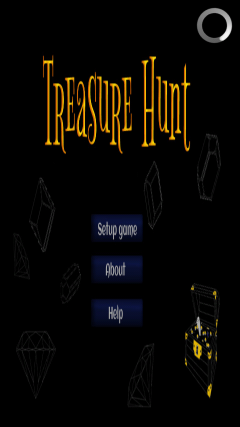
\includegraphics[width=2.5in]{snaps/splash} &
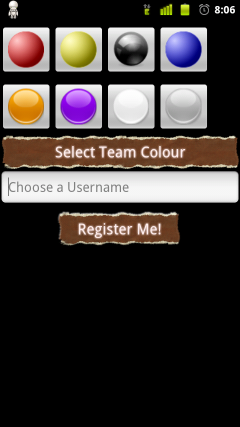
\includegraphics[width=2.5in]{snaps/user} &

\end{array}$
\end{center}
\caption{Spash Screen & Team Select}
\end{figure}

\begin{figure}[h]
\begin{center}$
\begin{array}{cc}
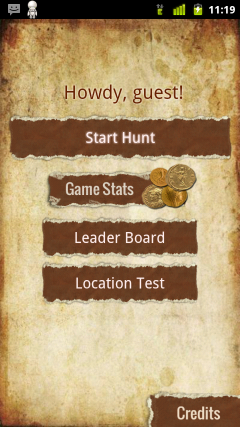
\includegraphics[width=2.5in]{snaps/3} &
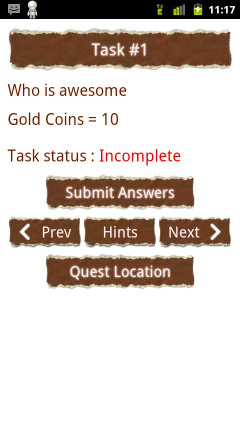
\includegraphics[width=2.5in]{snaps/4} 
\end{array}$
\end{center}
\caption{Main Menu & Task List}
\end{figure}

\begin{figure}[h]
\begin{center}$
\begin{array}{cc}
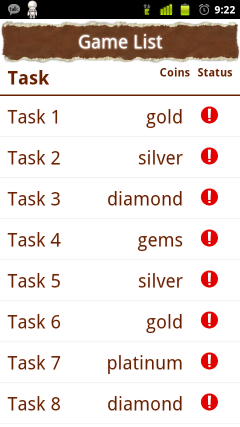
\includegraphics[width=2.5in]{snaps/5} &
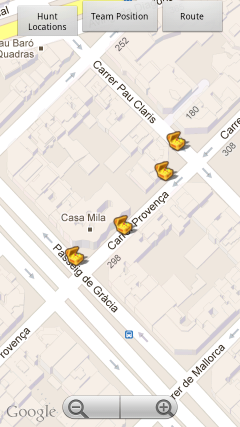
\includegraphics[width=2.5in]{snaps/6} 
\end{array}$
\end{center}
\caption{OverLays Map & Custom Location}
\end{figure}

\begin{figure}[h]
\begin{center}$
\begin{array}{cc}
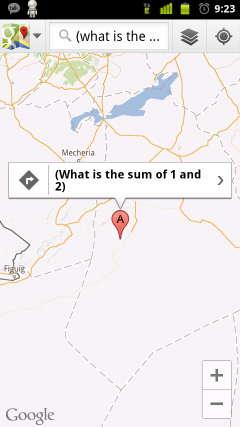
\includegraphics[width=2.5in]{snaps/7} &
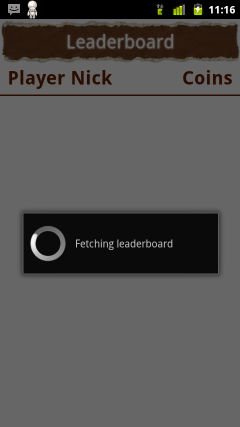
\includegraphics[width=2.5in]{snaps/8} 
\end{array}$
\end{center}
\caption{Async Loading using Simple Adapter}
\end{figure}

\begin{figure}[h]
\begin{center}$
\begin{array}{cc}
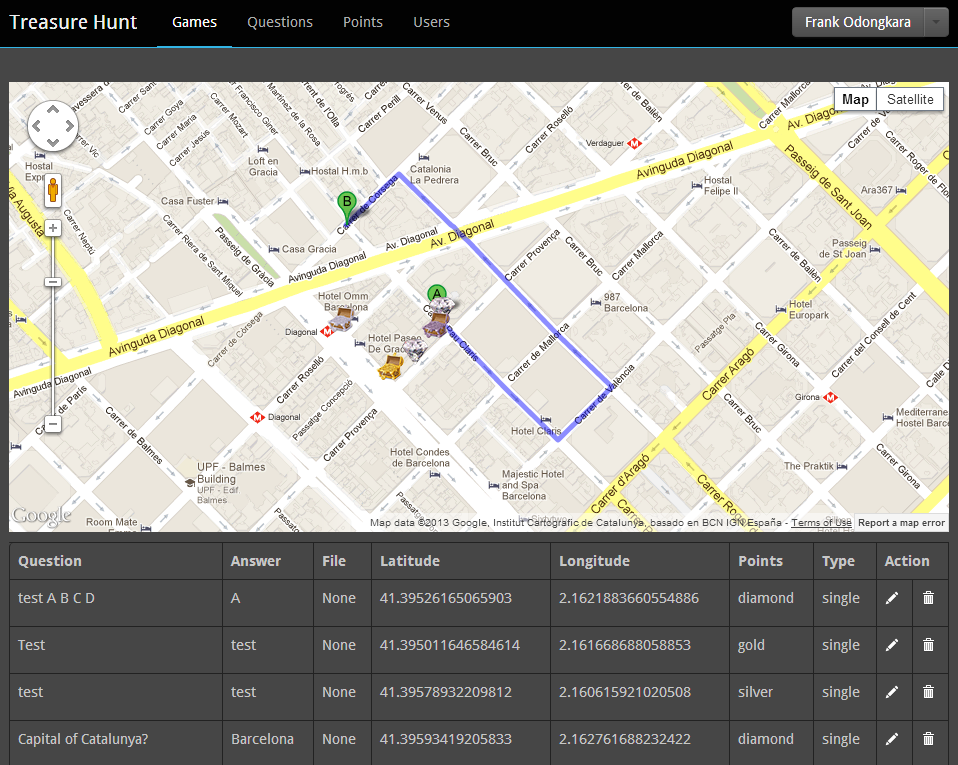
\includegraphics[width=2.5in]{images/maps} &
\end{array}$
\end{center}
\caption{Google Maps on Server }
\end{figure}





\chapter{Future Aspects}

Being build with the power of Cloud and Android this will have many uses , Its not long back when on April 1 2013 Google Released location where actual treasures were found by treasure hunters where other native people considered that as a April fools day Ha-ox. Implementing In Video on Google Customized Maps over Overlays and Custom route navigation with intelligent navigation is what will be released in the next release . The Application can be found on Google Play under the name of Treasure Hunt [Ankit APPS] \\

\chapter{Conclusion}

Treasure Hunting Game not only remains the concept of hunting treasures with maps but also integrates GPS function. With a designed route for treasure hunting, the students would not miss any places for treasures. During the process of game, students can participate in the activity and observe the environment in person and absorb the knowledge unconsciously. Meanwhile, students can learn how to apply GPS and the skills of reading maps to obtain the knowledge happily.








\end{adjustwidth}